\subsection{PPPoE}

The Internet connection on \gls{vlan} 600 uses \gls{pppoe} \cite{rfc2516} for tunneling its packages. The protocol requires the user to authenticate and then can provide encryption and compression for the connection. On the \glspl{cpe} being studied, the authentication mechanism of \gls{pppoe} is not really used for client authentication. Each customer is identified based on which port the copper or fiber cable connects to on the \gls{isp} side.

The \gls{pppoe} credentials are hardcoded on all \glspl{cpe} analyzed. The \gls{http} Management Interface explicitly instructs the user to set \texttt{cliente@cliente} as the username and \texttt{cliente} as the password, as seen in Figure \ref{figure:cpe_pppoe}.

\begin{figure}[h]
    \centering
    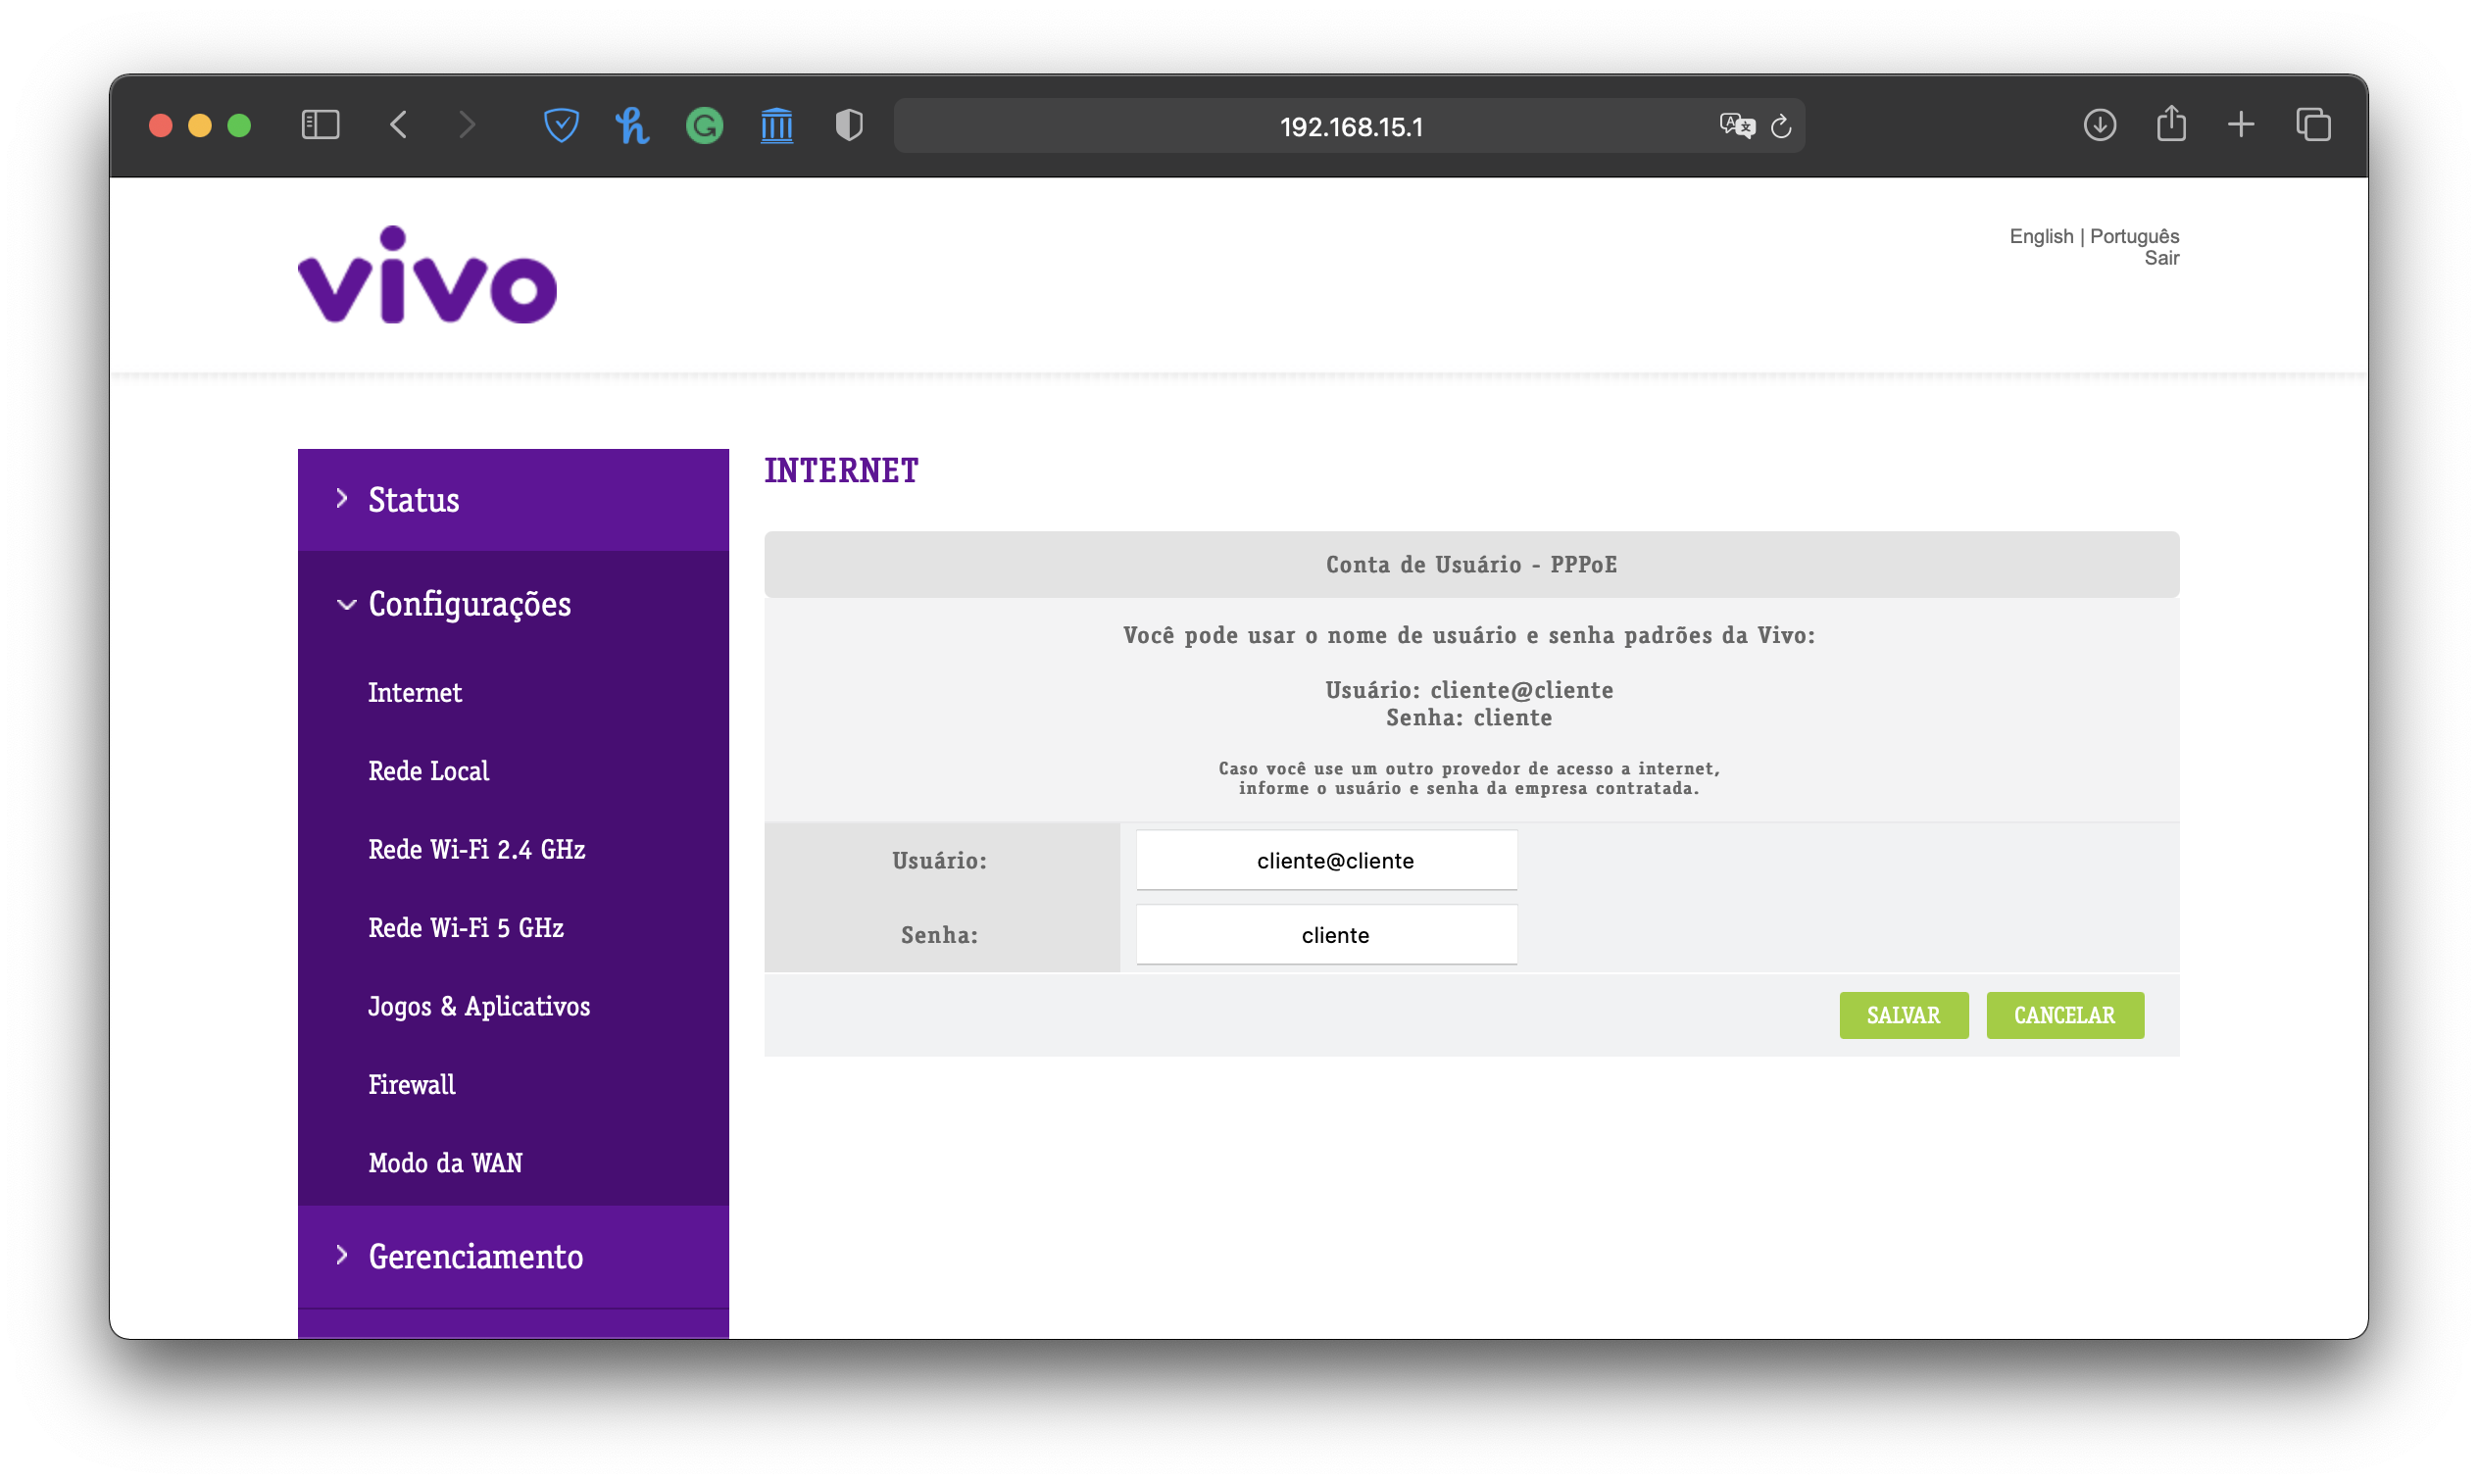
\includegraphics[width=\linewidth]{contents/configuration-analysis/pppoe/cpe-pppoe.png}
    \caption{\gls{pppoe} Settings on \gls{cpe}}
    \label{figure:cpe_pppoe}
\end{figure}

\FloatBarrier
